% 相机模型
% 投影|光轴|焦点|投影

\pentry{三维投影\upref{proj3D}, 图片坐标系\upref{imgFrm}}

\begin{figure}[ht]
\centering
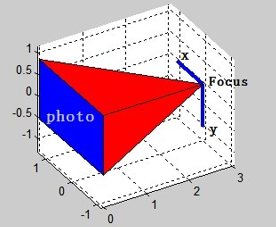
\includegraphics[width=5cm]{./figures/CamMdl_1.png}
\caption{相机坐标系} \label{CamMdl_fig1}
\end{figure}

从焦点出发, 穿过底片并与底片垂直的射线叫做\textbf{光轴}.

以焦点为原点, 光轴方向为 $z$ 轴, 图片的右方为 $x$ 轴, 下方为 $y$ 轴(注意这是常用的右手系\upref{RHRul}).

真实的相机和这里的相机模型存在误差, 通常需要将图片进行纠偏后才能得到符合模型的图像. 以后我们讨论的图像一般指纠偏后的图像.

注意图像的中点不一定是光轴和底片的交点.

相机参数: 焦距, 底片宽度, 底片高度, 光轴的图像坐标

相机的位置参数: 焦点的位置, 三个单位矢量在世界坐标系中的坐标(即旋转矩阵, 也可以使用四元数表示)

反过来, 若已知图片和相机位置和参数, 我们可以将图片上的每一点对应到以相机为起点的一条射线. 而至于这点具体在射线上的什么位置无从得知. 但如果我们从两个不同的位置拍摄同一点, 就可以通过两条射线的交点确定该点位置.

若已知相机参数, 我们可以通过图片中的任意两点确定它们关于相机的夹角(即两条射线的夹角).

\subsection{变换方程}
变换有 7 个自由度, 相机位置 3 个, 相机角度 3 个, 相机焦距 1 个.

一般形式为(推导: 根据相机模型结合立体几何)
\begin{equation}\label{CamMdl_eq1}
\leftgroup{
x' &= \frac{c_4 x + c_5 y + c_6 z + c_7}{c_1 x + c_2 y + c_3}\\
y' &= \frac{c_8 x + c_9 y + c_{10} z + c_{11}}{c_1 x + c_2 y + c_3}
}
\end{equation}
注意这里的 9 个常系数中只有 7 个是独立的. 所以理论上我们可以只用 4 个一般位置的点及它们在图片上的坐标解得所有的系数, 但这样方程就不是线性的了. 所以我们也可以假设 9 个系数都是独立的, 并用 6 个或以上一般位置的点得到 12 条(或以上) 关于 $c_i$ 的超定齐次线性方程组, 并利用超定来减小误差.

如果我们不仅需要得到变换公式, 还需要从这些系数里面得到相机的位置和朝向, 那么我们可以从立体几何的角度出发, 例如见长方形相机定位法\upref{RecCam}. 但这样我们需要的 4 个点就必须是长方形的四个顶点而不是任意点.

\subsection{平面到平面的变换}
注意\autoref{CamMdl_eq1} 不存在逆变换, 因为我们把空间中的点投影到平面上时丢失了景深的信息. 但如果我们限制所有空间点 $(x, y, z)$ 都在某个平面上(不失一般性, 假设它们在 $x$-$y$ 平面上), 那两个平面上的点就有一一对应的关系.

\begin{equation}
\leftgroup{
x' &= \frac{c_4 x + c_5 y + c_6}{c_1 x + c_2 y + c_3}\\
y' &= \frac{c_7 x + c_8 y + c_9}{c_1 x + c_2 y + c_3}
}
\end{equation}
可以证明其逆变换也有相同的形式, 虽然这并不显然.
